%%%%%%%%%%%%%%%%%%%%%%%%%%%%%%%%%%%% Chapter Template

\chapter{Caso de Estudo - \textit{Living Labs'}} 	% Main chapter title
\label{Chapter3} 		% For referencing the chapter elsewhere, usage \ref{Chapter6}

O modelo de \textit{"Living Lab' "} ou (Laboratório Vivo) emerge como uma abordagem colaborativa entre os \textit{stakeholders} do setor empresarial, setor público e privado, trabalhando em conjunto para criar, testar e validar ideias num ambiente real, ou seja, numa cidade inteligente.
O conceito de \textit{"Living Labs' "} tem vindo a ganhar destaque no contexto das cidades inteligentes, especialmente no que diz respeito à logística urbana.
Um exemplo notável deste caso de estudo é o projeto  (\gls{smile}),que já foi referido no capítulo anterior \ref{Chapter2} no artigo V \cite{NAVARRO2016314}.


Estes laboratórios vivos são ambientes reais onde novas tecnologias, serviços e modelos económicos, podem ser testados e avaliados em condições reais de uso.
No âmbito da logística urbana, os \textit{"Living Labs' "} oferecem uma plataforma para experimentar soluções inovadoras que visam melhorar a eficiência, sustentabilidade e qualidade de vida nas cidades.

A associação internacional sem fins lucrativos \gls{enoll} \textit{European Network of Living Labs}, enquanto entidade representante internacional desta rede, tem sede em Bruxelas, na Bélgica no centro da \gls{ue}, promove novos projetos e congressos para promover laboratórios vivos que promovam a inovação aberta e a cocriação em diversos setores.

A \gls{fig} \ref{fig:living_lab} ilustra os diferentes setores dos membros da \gls{enoll} \cite{EuropeanNetworkofOpenLivingLabs2025}, que é a maior rede de \textit{"Living Labs' "} na Europa.
\begin{figure}[H]
    \centering
    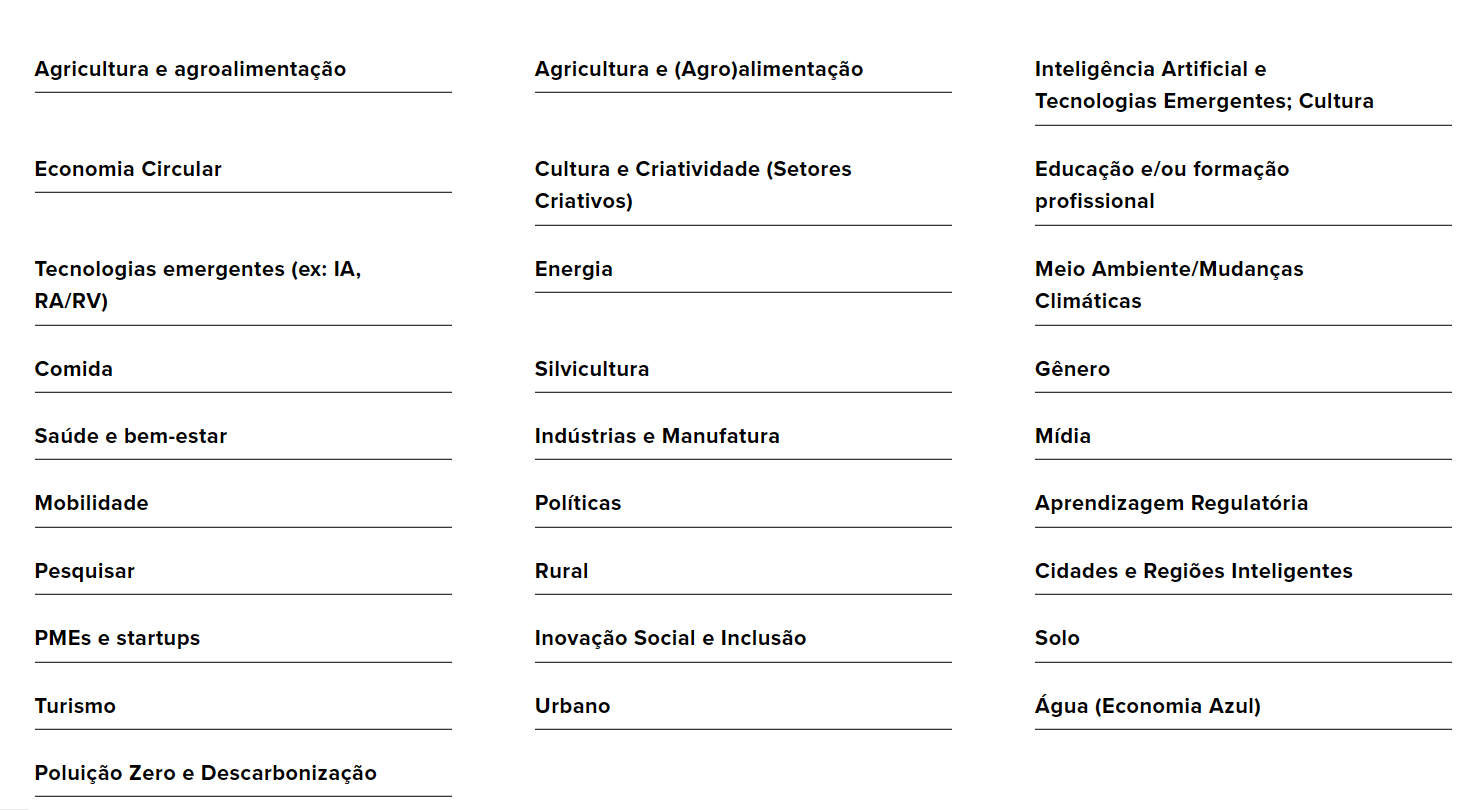
\includegraphics[width=1.0\textwidth]{figures/caso-de-estudo/Living Labs Areas de Atuação.png}
    \caption{Setores dos membros da \gls{enoll} citado em:  \cite{EuropeanNetworkofOpenLivingLabs2025}.}
    \label{fig:living_lab}
\end{figure}

Estes setores, têm como infraestruturas críticas principais na \gls{fig} \ref{fig:aidrivenoptimization} \cite{articleadd}.
\begin{figure}[H]
	\centering
	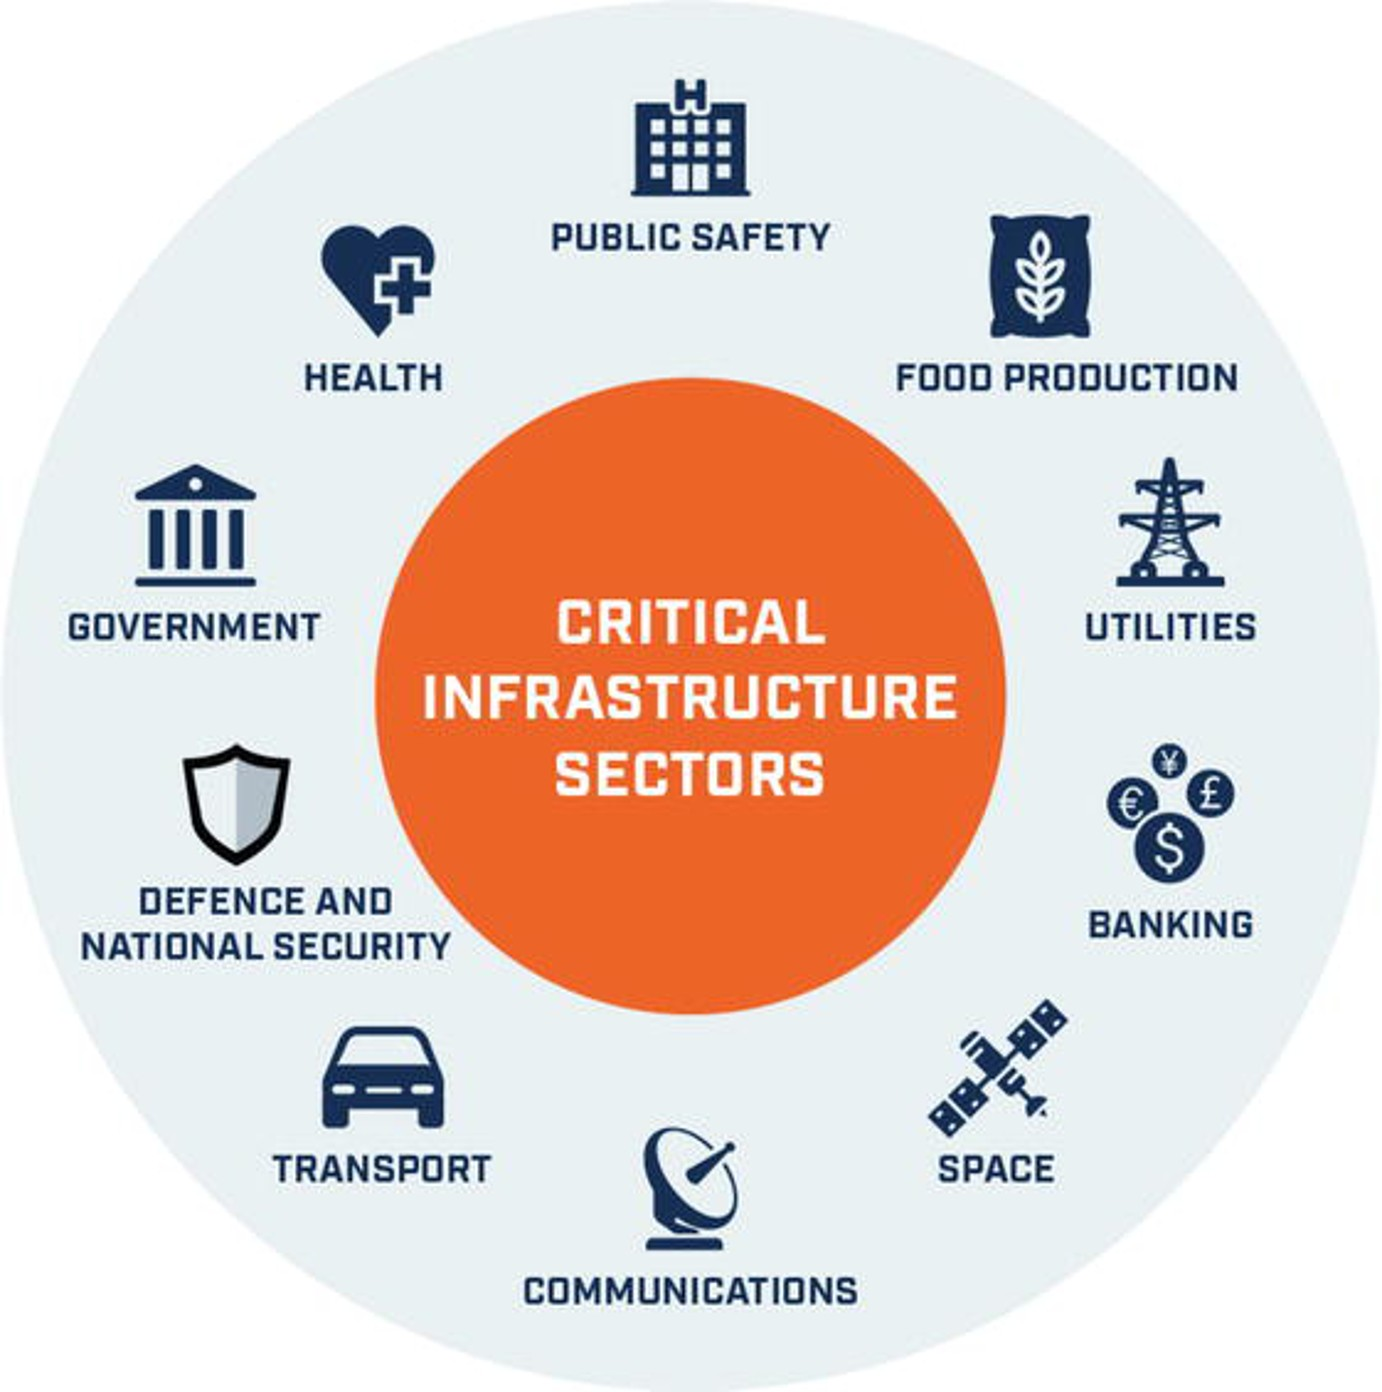
\includegraphics[width=0.85\textwidth]{figures/setorescominfraestruturascriticas.jpg}
	\caption{Infraestruturas críticas em diferentes setores, citado em: \cite{articleadd}.}
	\label{fig:aidrivenoptimization}
\end{figure}

A \gls{civitas} é uma outra iniciativa da \gls{ue}, que tem como objetivo desenvolver e implementar soluções de mobilidade urbana sustentável em cidades europeias \cite{CIVITAS_2025}.
Este projeto é feito por meio de uma rede de cidades, para cidades, dedicada à mobilidade urbana sustentável na \gls{ue}.


Aproximadamente 70\% dos cidadãos da \gls{ue} vivem em áreas urbanas, onde os efeitos das emissões de gases de efeito estufa provenientes do transporte rodoviário, ferroviário, aéreo e marítimo,  entre outros, representam um quarto das emissões totais da \gls{ue} \cite{CIVITAS_2025}.
A ideia central da \gls{civitas} é criar uma comunidade de cidades que partilham sustentabilidade e inovação umas com as outras contribuindo para a adesão de políticas da \gls{ue}.
A \gls{fig} \ref{fig:civitas_cities} apresenta as cidades participantes na iniciativa \gls{civitas} até 2025 \cite{CIVITAS_2025}.
\begin{figure}[H]
    \centering
    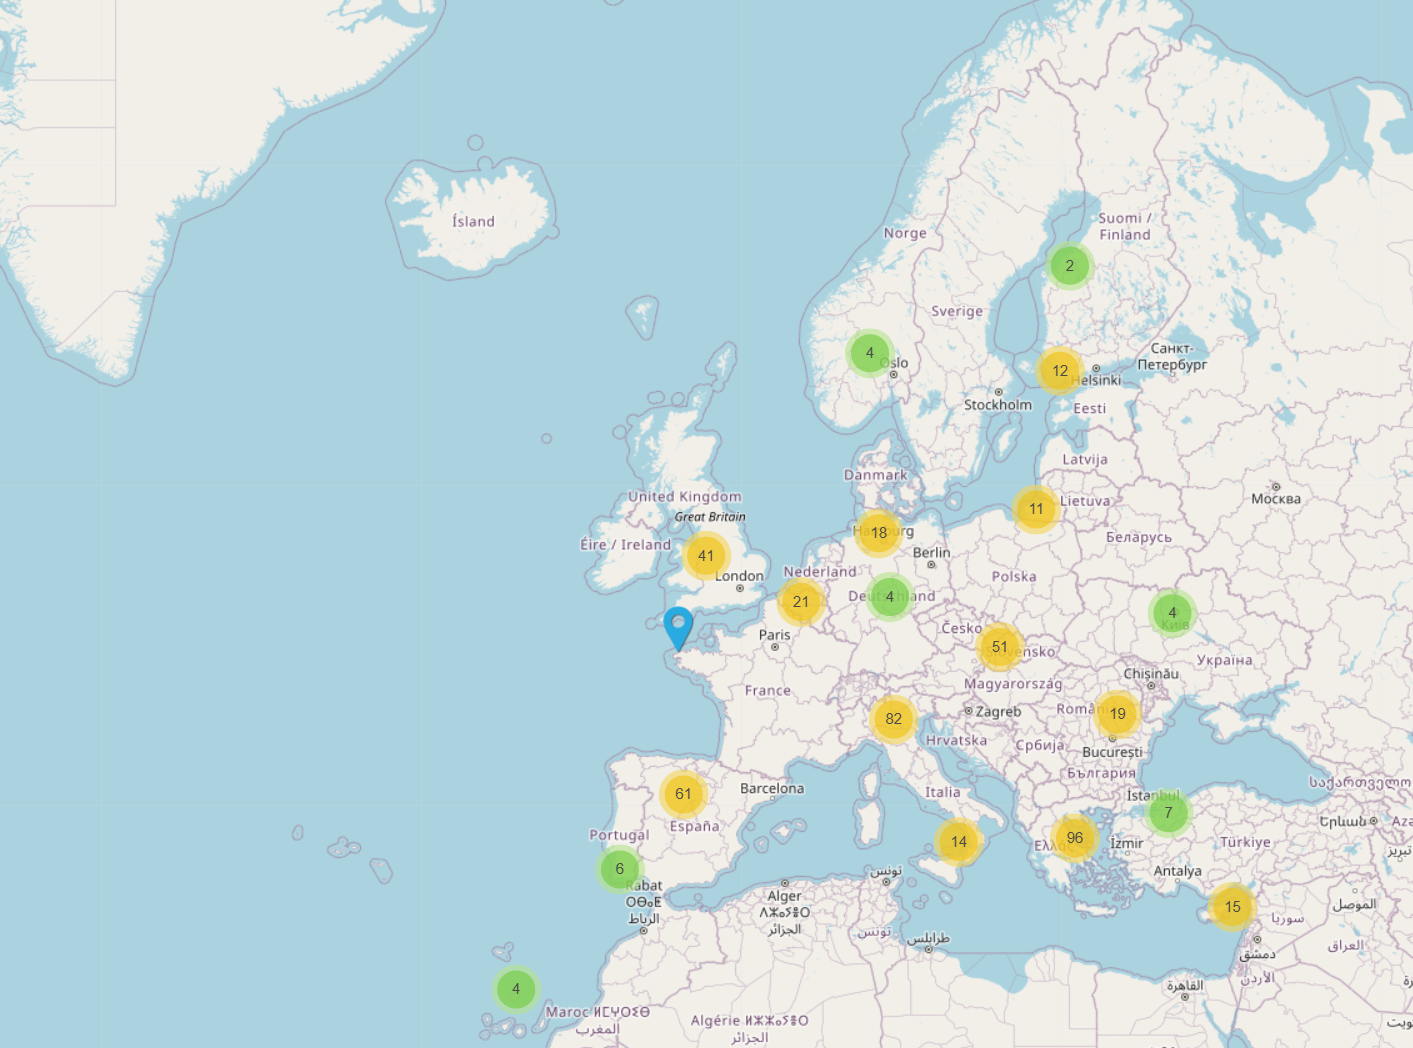
\includegraphics[width=1.3\textwidth]{figures/participantes-civitas.png}
    \caption{Cidades participantes na iniciativa \gls{civitas} até 2025, citado em: \cite{CIVITAS_2025}.}
    \label{fig:civitas_cities}
\end{figure}
A tabela abaixo resume as vantagens e desvantagens dos \textit{"Living Labs' "} no contexto da logística urbana em cidades inteligentes.
\begin{table}[H]
\centering
\footnotesize
\begin{tabular}{|p{8cm}|p{8cm}|}
\hline
\textbf{Vantagens} & \textbf{Desvantagens} \\
\hline
Ambiente real para testar soluções inovadoras & Custo elevado de implementação e manutenção de infraestruturas \\
\hline
Promove colaboração entre \textit{stakeholders} nos setores (público, privado, académico) & Necessidade de leis de governação e regulamentação aprovadas pela Assembleia de República de cada país e da \gls{ue} \\
\hline
Reduz risco de falhas em larga escala (testes controlados em regiões prontas para projeto-piloto) & Escalabilidade limitada a regiões piloto apenas \\
\hline
Facilita a co-criação e inovação aberta a novas tecnologias & Dependência de financiamento público/privado de cada país \\
\hline
Permite recolha de dados em tempo real para análise de dados em tempo real & Complexidade na integração de diferentes sistemas, necessitam de se comunicarem uns com os outros \\
\hline
Contribui para sustentabilidade e qualidade de vida urbana & Resistência cultural e falta de adesão dos civis de maior idade ou governos com ideias conservadoras \\
\hline
Acelera validação de tecnologias emergentes nas cidades & Risco de resultados não replicáveis fora do projeto-piloto \\
\hline
Cria oportunidades para parcerias público-privadas e cofinanciamentos da \gls{ue} & Tempo elevado para alinhar interesses e aprovar regulamentos necessários para aprovação \\
\hline
Favorece aceitação social ao envolver cidadãos & Vulnerabilidade a mudanças políticas que podem interromper projetos como guerras civis ou crises econômicas \\
\hline
\end{tabular}
\caption{Vantagens e desvantagens do modelo \textit{"Living Labs '"} aplicado a cidades inteligêntes.}
\label{tab:livinglabs}
\end{table}
